\documentclass[a4paper]{article}
\usepackage{geometry}
\geometry{left=3.5cm,right=3.5cm,top=3.5cm,bottom=3.5cm}
\usepackage{amsmath, amssymb}
\usepackage{graphicx}
\usepackage{subfigure}
\usepackage{pdfpages}

\usepackage{xeCJK}
\setmainfont{Times New Roman}
\setCJKmainfont[BoldFont=SimHei,ItalicFont=KaiTi]{SimSun}

\usepackage{indentfirst}
\setlength{\parindent}{2em}

\usepackage{fancyhdr}
\pagestyle{fancy}
\usepackage{lastpage}
\rhead{Page \thepage{} of \pageref{LastPage}}
\lhead{A25}
\cfoot{}
\renewcommand{\headrulewidth}{0pt}
\renewcommand{\figurename}{图}
\renewcommand{\tablename}{表}

\headheight 14pt

\usepackage{float}

\renewcommand\baselinestretch{1.2}
\begin{document}

\includepdf[addtotoc={1,section,1,title in toc,cc},pages=3-4,offset=0cm 0cm]{title.pdf}

\part*{摘要}
\textit{本文从中国国情出发,结合年龄、地区、受教育水平等因素,借鉴了已有的人口学模型,逐步建立并完善了一个动态变动的人口模型。着眼于计划生育新政策带来的影响,本文着重讨论了计划生育政策下多胎生育受到的限制,以及二胎政策开放与否在人口结构、教育资源、劳动力供给等方面的差异。通过对于一些研究计划生育的论文的分析,反思了该模型的不足与缺陷,并提出了其合理性与优势面。最后,通过建立适当简化的养老金模型,探讨了二胎政策是否能够真正缓解养老基金日益短缺的问题,并给出了可能的解决方案。}

\part{目录}
\tableofcontents

\part{引言}
1957年2月,在最高国务会议第十一次(扩大)会议上,著名经济学家、北京大学校长马寅初就“控制人口”问题发表了自己关于控制中国人口数量的主张。同年6月,马寅初将《新人口论》作为一项提案,提交一届人大四次会议(全文发表于7月5日《人民日报》)。《新人口论》从10个方面论述了为什么要控制人口和控制人口的重要性与迫切性,以及如何控制人口等问题。\\
\indent
1971年,国务院下发《关于做好计划生育工作的报告》。这一报告是中国整个计划生育工作的真正起点。从此,计划生育真正成为国家计划的一部分,成为了名副其实的“计划”生育。政府开始通过逐级下达的层层指标,严格控制人口出生。同时,全国各级政府对计划生育的资金投入也明显增加。\\
\indent
开展计划生育的30多年来,我国经济水平飞速增长。但与此同时,我国的生育水平却在逐步下降,综合生育率由1981年的2.61降至2014年的1.55\footnote{维基百科编者. 总和生育率[G/OL]. 维基百科, 2016(20160429)[2016-05-02]. https://zh.wikipedia.org/w/index.php?title=\%E6\%80\%BB\%E5\%92\%8C\%E7\%94\%9F\%E8\%82\%B2\%E7\%8E\%87\&oldid=39936095.},远低于生育更替水平\footnote{数据来源于世界银行数据库; 在出生性别比例正常情况下,国际上普遍认为生育更替水平为2.05-2.1。}。从1980年9月25日中共中央发表《计划生育公开信》开始,该政策已执行35年。其间,人口专家曾于2004年、2009年先后集体谏言,建议中央及早取消独生子女政策,但并未被采纳。\\
\indent
在经历了迅速从高生育率到低生育率的转变之后,我国人口的主要矛盾已经不再是增长过快,而是人口红利消失、临近超低生育率水平、人口老龄化等问题。国内20多位顶尖人口学者历经两年的研究指出,我国的人口政策亟待转向,尤其是生育政策应该调整。之前,以独生子女政策为核心内容的我国计划生育政策,自20世纪80年代开始严格推行。其间略有微调,如于2011年11月25日放开“双独二胎”(夫妻双方为独生子女,可以生育第二个孩子),及部分省份农村地区实施的“一孩半”政策(第一个孩子为女孩,可生育第二个孩子)等。\\
\indent
在2013年11月15日放开“单独二胎”(夫妻一方为独生子女,可以生育第二个孩子)后,新生儿数量虽然得以因政策的实施而增长,但仍然低于先前预期的会申请养育二胎的人数。所以为了解决自计划生育实施以来所出现的一系列问题,2015年10月,中共十八届中央委员会第五次全体会议公报指出:促进人口均衡发展,坚持计划生育的基本国策,完善人口发展战略,全面实施一对夫妇可生育两个孩子政策,积极开展应对人口老龄化行动,也就是人们常说的“全面二孩”政策。\\
\indent
二孩政策究竟能够对人口老龄化现象产生多大影响,我们所谓的“80后”、“90后”又是否成为了唯一的一代独生子女,诸多问题在推出二孩政策后接踵而来。这些问题的答案,与全国人群受教育程度、城镇化比例和年龄分布随着时间推移的变化是分不开的。
\part{假设}
2001年邦加茨 (Bongaarts)提出生育水平与生育意愿关系的理论,认为从人们的生育意愿到实现生育行为结果这一过程会受一系列因素的影响,包括非意愿生育($F_u$)、替补效应($F_r$)、性别偏好($F_g$)、进度效应($F_t$)、不孕效应($F_i$)和竞争效应($F_c$)等。\footnote{J. Bongaarts, “\textit{Fertility and Reproductive Prefernces in Post-Transitional Societies}”, Population and Development Review, vol.27, no.2, 2001, pp.260-281}2003年摩根(Morgan)基于此理论构造出模型\footnote{S. P. Morgan, “\textit{Is Low Fertility a Twenty-First-Century Demographic Crisis?}” Demography, vol.40, no.4, 2003, pp.589-603}$TFR=F_u \cdot F_r \cdot F_g \cdot F_t \cdot F_i \cdot F_c \cdot IP$,其中$IP$为理想子女数。本文出于简化模型的考虑,将非意愿生育($F_u$)、性别偏好($F_g$)与不孕效应($F_i$)归结为孕龄妇女所处地区(城、乡、镇),而将替补效应($F_r$)、进度效应($F_t$)、和竞争效应($F_c$)归结为孕龄妇女所接受的教育程度。如此考虑的原因有两个,一个是Morgan所提出的模型中参数难以量化,其次是不同年龄段妇女生育情况与其所处地区、所受教育程度联系的数据可以在中国第六次人口普查的长表数据中得到,这是我们赖以建立模型最合理也是最有效的数据。\\
\indent
其次,在我们的模型中,我们认为全国平均有10\%的妇女一生不会生育子女。2002年,上海市妇联针对全市家庭状况所作的一项调查显示,丁克家庭已经占到上海家庭总数的12.4\%。事实上,随着经济发展与观念的改变,丁克家庭的比例仍在逐步上升。考虑到上海的丁克家庭比例可能高于其他大多数地区,所以我们在模型计算时认为始终有10\%的妇女一生内都不会生育子女。\\
\indent
一个饱受争议的方面是性别比。有论文\footnote{马秀文、石少刚:《浅谈我国男女比例失调的法律思考》,《企业导报》2011年第21期,第238-239页}指出,中国新生儿男女比严重失调与计划生育制度有着不可分离的影响,其中一个很重要的原因是农村重男轻女思想严重,从而导致新出生男女比例不均衡。但根据《中国统计年鉴》的数据,自1978年至今,中国的男女比例始终处于一个稳定的状态;同时“数据显示,农村妇女数量已经十分接近2.0个子女了,放不放开生育政策对她们没有什么实际意义了”\footnote{黄润龙:《“全面二孩政策”与人口长期均衡发展》,《唯实》2016年第2期,第58页}。我们有理由相信,二孩政策的放开并不会对中国平均男女比产生重大的影响;所以在模型的计算中,我们用第六次人口普查数据的男女比例来当作中国若干年都将维持的男女比例(同时也不考虑男女在相同年龄死亡率的差异)。
\part{人口增长的简单模型}
\label{simple_model}
\section{引述}
人口的变动,自人类的历史追溯而来也有相当长的历史了。不可否认的是,除了疾病、战争等因素的影响以外,几乎毫无例外地、人类数量是在不停地增长的,而且速度越来越快:1804年人口总数刚刚抵达10亿人,而100多年后的1927年就增至两亿;此后增长一亿的时间更是缩短至33、15、13、12年\footnote{维基百科编者. 人口[G/OL]. 维基百科, 2016(20160221)[2016-05-02]. https://zh.wikipedia.org/w/index.php?title=\%E4\%BA\%BA\%E5\%8F\%A3\&oldid=39145999.} 。经济的发展、社会的安定都离不开对于人口增长的准确预测。\\
\indent
人类学发展至今,已经有过很多的人口模型与学说了。从最早的马尔萨斯线性人口模型,到考虑环境容纳量的Logistic 人口模型,其最为主要的两个考虑方面都是人口的出生与消亡。有所不同的是,马尔萨斯模型仅考虑不受环境约束的情况下,人能够以固定的比率无限繁衍;而Logistic 模型更加细致地考察了环境对于人口增长的影响。然而,仅仅考虑这两方面还是只能得到比较普适的结果,并不能真正地将其应用于中国的人口推演。\\
\indent
人口的生育率,既随着生产条件、医疗水平的提升而上升,也随着社会观念、教育水平的改变而变动。根据前面在假设中所提到的理由,我们在这个模型中主要着眼于地区差别、受教育水平的不同而对生育率产生的影响。
\section{模型概述}
人口的变动,和人口的产生与消亡这两方面是密不可分的。人口的增长,一方面会被人口的产生所促进,另一方面又会被人口的消亡所限制,所以是一个动态平衡的过程。大量新出生的人口在达到适育年龄的时候会对人口的增长起到促进作用;而相反地,当他们走向衰老乃至死亡的时候,又会加剧人口的减少。这也就是为什么控制人口均衡增长是如此的重要,而这个均衡一旦被打破后可能会在若干年后带来不可置信的后果。下面我们分别着手处理这两个问题。
\subsection{人口的衰老}
每个人都会随着时间的流逝而逐渐衰老,随后在某天离世。众所周知,死亡率是一个随着年龄而变化的数据;由于孩童抵抗力弱,易夭折,所以婴儿的死亡率较高,然后随着年龄的增长而下降。到40岁及以上时,由于人的身体机能下降而导致死亡率逐步回升。在人口年龄分布上便体现为青壮年人口比例最高。
\subsection{人口的出生}
各个年龄层次的适育妇女,都有可能在考察的时间段内生育:对于个人而言,这是一个概率性事件;但是对于群体而言,生育事件的随机性就被大量的人群基数所磨灭,成为一个比率。因此,一段时间内婴儿的出生数目,等于平均生育率乘上适育妇女的人数。但是由于地区与学历的不同,这些妇女对于生产意愿的态度不尽相同。为了简化问题,我们在简化模型中认为所在地区与教育程度带给人的影响是近似独立的,因此可以直接根据地区或是教育对平均生育率进行修正。在这种假设下,一段时间内婴儿的出生人数,就等于各年龄层的适育妇女乘上修正后的生育率之和。
\section{记号表}
	\begin{table}[H]
		\centering
		\caption{人口增长的简单模型}
		\label{simple_symbol}
		\begin{tabular}{cccc}
			\hline
			符号		&	含义									&	相关的其他参数	&	备注 \\
			\hline
			$a$			&	年龄									&	& \\							&&&$e_0$:小学及以下\\
			$e$			&	受教育水平(枚举量)	&									& 	$e_1$:中学	\\	&&&$e_2$:大学及以上	\\&&&$r_0$:城\\
			$r$			&	地区(枚举量)				&									& $r_1$:镇	\\	&&&$r_2$:乡	\\
			$t$			&	考察的时间段					&	& \\
			$I$			&	出生婴儿数						&	$e,r,t$		& \\
			$N$			&	总人口数							&	$a,e,r,t$ & \\
			$W$		&	女性人数							&	$a,e,r,t$	& \\
			$\beta$	&	生育率								&	$a,e,r$	& \\
			$\delta$	&	平均死亡率						&	$a$			& \\
			$\lambda$	&	修正系数						&	$a,e,r$	& \\
			$\mu_p$& 男女比例								&	& \\
			\hline
		\end{tabular} \\
	\end{table}
\section{数据的引用}
	\begin{table}[H]
		\centering
		\caption{2010各地出生婴儿数与其母亲受教育程度情况}
		\label{simple_data}
		\begin{tabular}{c|ccc}
			$I(r_k, e_l, 2010)$		&	$e_0$		&	$e_1$		&	$e_2$ \\
			\hline
			$r_0$							&	16877		&	19167		&	99670	\\
			$r_1$							&	24683		&	168432	&	25719	\\
			$r_2$							&	136021	&	480524	&	13587	\\
		\end{tabular}
	\end{table}
\section{方程的建立}
首先,考虑人口的自然衰老:
	\begin{equation}
		\label{simple_people_aging}
		N(a+1,t+1) = N(a,t) \cdot (1-\delta (a))
	\end{equation}
这里$\delta (a)$指的是$a$岁人口的平均死亡率。\\\\
\indent
再考虑所有地区,由受各种教育水平的妇女生育的婴儿数:
	\begin{equation}
		\label{simple_people_birth}
		N(0,t+1) = \sum_{r_k} \sum_{e_l} I(r_k, e_l, t)
	\end{equation}
这里$I(r_k, e_l, t+1)$表示在$t$这个考察时间段内,在$r_k$地区,受到$e_l$教育水平的妇女生育的婴儿数目。\\\\
\indent
考察$I(r_k, e_l, t)$是由各个不同年龄阶段的适龄妇女所生育的:
	\begin{equation}
		\label{simple_tiny_people_birth}
		I(r_k, e_l, t) = \sum_a \beta(a, r_k, e_l)W(a, r_k, e_l, t)
	\end{equation}
这里$\beta(a, r_k, e_l)$是$r_k$地区,受到$e_l$教育水平的妇女的生育率,$W(a, r_k, e_l, t)$是这段时间这类妇女的总人数。\\\\
\indent
总人口数与总女性数之间存在着简单的比例关系:
	\begin{equation}
		\label{simple_ratio_people_female}
		N(a,r,e,t) = W(a,r,e,t) \cdot (1+\mu_p)
	\end{equation}
这里$\mu_p$表示的是男性与女性人数的比例。\\\\
\indent
教育水平与地区对于生育率的修正,即$\beta(a, r_k, e_l)$,是这样构成的:
	\begin{equation}
		\label{simple_birthrate}
		\beta(a, r_k, e_l) = \overline{\beta(a)} \cdot \lambda_{r_k} \cdot \lambda_{e_l}
	\end{equation}
其中$\overline{\beta(a)}$是平均生育率,$\lambda_{r_k}$与$\lambda_{e_l}$分别是地区与教育水平分别对于生育率的修正;为了记号上的方便,令$\lambda_b$为生育修正参数矩阵, 其中
	\begin{equation}
		\label{simple_birthrate_factor}
		\lambda_b(r_k,e_l) = \lambda_{r_k} \cdot \lambda_{e_l}
	\end{equation}
\\\\
\indent
在进一步完善模型之前,我们给出$\lambda_b(r_k,e_l)$的计算公式与结果。事实上,根据等式\ref{simple_tiny_people_birth}与等式\ref{simple_birthrate},我们可以立即得到:
	\begin{equation}
		\label{simple_lambda_b_calc}
		\lambda_b(r_k,e_l) = \frac{I(r_k, e_l, t)}{\sum_a \overline{\beta(a)} W(a, r_k, e_l, t)}.
	\end{equation}
利用表\ref{simple_data}中的数据,代入$t=2010$,我们得到了$\lambda_b(r_k,e_l)$的具体结果,见表\ref{simple_lambda_b_value}:
	\begin{table}[H]
		\centering
		\caption{生育修正参数$\lambda_b$}
		\label{simple_lambda_b_value}
		\begin{tabular}{c|ccc}
			$\lambda_b(r_k,e_l)$	&	$e_0$	&	$e_1$	&	$e_2$	\\
			\hline
			$r_0$								&	0.802	&	0.796	&	0.630	\\
			$r_1$								&	1.013	&	1.104	&	0.588	\\
			$r_2$								&	1.063	&	1.343	&	0.445	\\
		\end{tabular}
	\end{table}
在这个模型下,我们可以给出中国人口增长的一个粗略的估计(图\ref{simple_graph})。
	\begin{figure}[htbp]
		\centering
		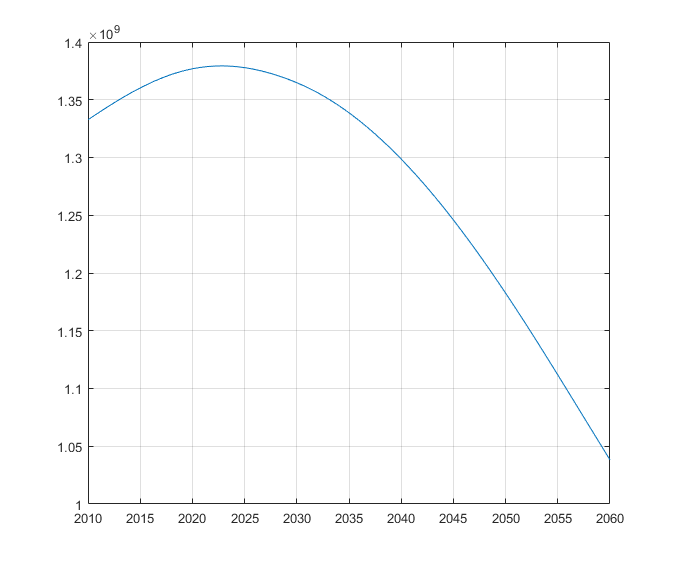
\includegraphics[width=10cm]{pics/simple_1.png}
		\caption{简单模型对中国人口的估计}
		\label{simple_graph}	
	\end{figure}
\section{小结}
我们可以看到,如果将公式\ref{simple_birthrate_factor}代入表\ref{simple_lambda_b_value}的数据中,并不能解得地区与教育程度对于生育率的修正(因为表\ref{simple_lambda_b_value}中有9个数据,而修正参数仅有6个)。这个结论是较为显然的,因为生育率最高的是农村地区受过中等教育的妇女,这与修正参数简单相乘得到生育率的计算方式是不符的。换言之,所在地区与教育程度对于生育率的影响并非近似独立,而是会有一个交互的作用。所以在后面的讨论中我们摒弃公式\ref{simple_birthrate_factor},而是直接使用生育修正参数矩阵$\lambda_b(r_k,e_l)$来进行计算。对于这两个因素交互的作用,我们会在后面的第\ref{pipan}章报告研究中作进一步的讨论。
	
\part{人口增长模型修正与应用}
\section{假设}
在2.1的引述中我们提到了,我们所构建的模型应该要结合中国当今实际现状加以完善。但显然之前的简单模型中并没有考虑到这些因素,所以我们要在下面的模型修正中引入一定的中国现状。\\
\indent
从中国自身的情况考虑,人口的变化主要还有以下几个方面:
\begin{itemize} 
\item \textbf{二胎乃至多胎} 中国人“多儿多女”的观念促使他们多生很多孩子,特别是在农村地区缺乏农业劳动力的地区,也许多生一个孩子会略微加重其花费在抚养上的成本(甚至可能只是多添置一副碗筷),但却意味着更多的劳动力。于是多胎对于农村地区的吸引力不可忽视。
\item \textbf{计划生育政策} 正如引言所说,1981年开始实施的计划生育政策虽然遏制了当时过快上升的人口增长,但是推行至今,已成为中国孕育新生人口的阻力(可参考\ref{simple_graph})。之前的三十年来所累计的少出生的四亿人口,导致当今中国人口的年龄分布失衡。这在简单模型所得的图1中可以得到体现。
\item \textbf{全国范围内的流动人口} 眼下,“农民工进城”已是一个越来越不可忽视的社会问题。越来越多的农村人员转移至城镇务工就业,甚至携妻带子在城镇常住。但在城镇居住意味着要承担更高的教育支出和生活花销,这就会影响他们对于生育的观念。
\item \textbf{计划生育政策的放开} 马瀛通等(1986)针对中国计划生育政策实践提出年龄一孩次递进预测模型,该模型已经比较成功地用于人口预测与规划、计划生育奖励扶助、特别扶助制度目标人群等预测研究中,并得到长期、多次的实践检验。\footnote{王广州:《生育政策调整研究中存在的问题与反思》,《中国人口科学》2015年第2期,第5页}
\end{itemize}
\section{记号表}
	\begin{table}[H]
		\centering
		\caption{人口增长简单模型的修正}
		\label{amend_symbol}
		\begin{tabular}{ccc}
			\hline
			符号				&	含义																&	相关的其他参数	\\
			\hline
			$p_i$				&	期望生育$i$胎的妇女比例							&	$a$			\\
			$I_i$				&	作为第$(i+1)$胎出生的婴儿数目				&	$e,r,t$		\\
			$W_i$				&	生育了$i$个孩子的妇女数目						&	$a,e,r,t$	\\
			$\beta_i$		&	已生育$i$胎妇女的生育率							&	$a,e,r$	\\
			$\eta_a$		&	$a$岁已育一胎妇女的相对生育意愿			&	\\
			$\lambda_i$	&	已生育$i$胎妇女受到政策阻力修正因素	&	\\
			$\nu_r$	&	从$r_2$到$r_1$、$r_1$到$r_0$的地区迁移率				& \\
			$\nu_e$	&	从$e_2$到$e_1$、$e_1$到$e_0$的受教育水平迁移率	& \\
			\hline
		\end{tabular}
	\end{table}
\section{数据的引用}
	\begin{table}[H]
		\centering
		\caption{修正模型所涉及的参数}
		\label{amend_data}
		\begin{tabular}{ccc}
			\hline
			参数				&	值			&	含义 \\
			\hline
			$\alpha_p$	&	0.0057	& 2010年人口增长率	\\
			$\mu_c$			&	0.4523	&	2015年全国农村人口占总人口比例	\\
			$\mu_h$		&	0.1153	&	2015年受过高等教育的人数占总人数比例	\\
			\hline
		\end{tabular}
	\end{table}
\textbf{剩下的就直接甩链接。}
\section{模型的修正}
\subsection{依据生育情况区分妇女}
首先,适育妇女数,依照她们已生育孩子的数目,可分为$W_0$、$W_1$、$W_2$这三类,分别表示未生孩子、已生一个孩子与生了两个及以上的妇女数目。在这样的分类下,等式\ref{simple_tiny_people_birth}将被修正为如下带有下标的形式:
	\begin{equation}
		\label{amend_tiny_people_birth}
		I_i(r_k, e_l, t) = \sum_a \beta_i(a, r_k, e_l)W_i(a, r_k, e_l, t)
	\end{equation}
这里$I_i$是作为第$(i+1)$胎出生的婴儿数目,而$W_i$是生育过$i$胎的妇女数目。\\\\
\indent
同时,由于计划生育政策,已生育的妇女将会受到较大的政策阻力,因此她们的生育率将会减小。这一点反应在模型上是通过参数对方程进行调节的:
	\begin{equation}
		\label{amend_birthrate}
		\beta_i(a, r_k, e_l) = \overline{\beta(a)} \cdot \lambda_i \cdot \lambda_b(k,l)
	\end{equation}
其中$\lambda_i$是已生$i$胎妇女受到政策阻力的修正因数。\\\\
\indent
考虑在放开二胎政策之前,对于已生育的妇女而言,再生育的政策阻力应当是一致的。为了得到政策阻力的量化情况,我们采用数据拟合的手段。考虑$\lambda_i$具有如下的形式:
	\begin{eqnarray} \lambda_i=
		\label{amend_lambda_i_form}
		\begin{cases}
		(3-\lambda_{policy})	&	i=0	\cr	\lambda_{policy}	&	i=1	\cr	\lambda_{policy}	&	i=2
		\end{cases}
	\end{eqnarray}
这里参数$\lambda_{policy}$是由再分法确定的,使得人口增长率符合2010年人口增长率$\alpha_p$。拟合结果如表\ref{amend_lambda_i_value}所示。
	\begin{table}[H]
		\centering
		\caption{$\lambda_i$拟合结果}
		\label{amend_lambda_i_value}
		\begin{tabular}{c|ccc}
			参数	&	$\lambda_0$	&	$\lambda_1$	&	$\lambda_2$	\\
			\hline
			值		&	 1.92	&	0.54	&	0.54	\\
		\end{tabular}
	\end{table}
\indent
在第一次修正后,中国人口增长趋势大致如图\ref{amend_1}所示。\\
	\begin{figure}[htbp]
		\centering
		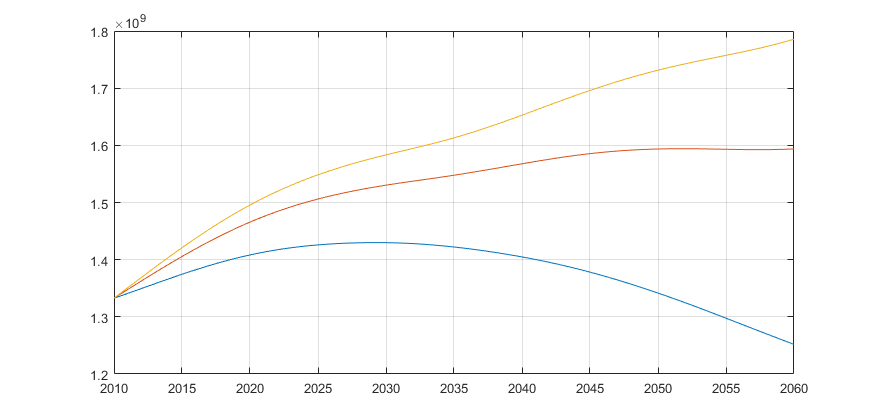
\includegraphics[width=10cm]{pics/amend_1.png}
		\caption{第一次修正后中国人口增长趋势预测}
		\*{蓝线:对应于计划生育}\\
		\*{红线:类似于放开二胎}\\
		\*{黄线:对应于自然生育} 
		\label{amend_1}	
	\end{figure}
\subsection{考虑人口的地域与教育水平的迁移}
随着时间的推移,人口逐渐向城市靠拢,同时由于自身的不断学习,受教育水平也在不断提升。这两个方面的迁移由以下的方程组来描述:
	\begin{equation}
	\left\{	
		\begin{aligned}
			\label{amend_migrate}
			N'(a,r_0,e_l,t+1) &= N(a,r_0,e_l,t+1) + \nu_r \cdot N(a,r_1,e_l,t+1)\\
			N'(a,r_1,e_l,t+1) &= (1 - \nu_r) N(a,r_1,e_l,t+1) + \nu_r \cdot N(a,r_2,e_l,t+1)\\
			N'(a,r_2,e_l,t+1) &= (1 - \nu_r) N(a,r_2,e_l,t+1)\\
			N''(a,r_k,e_0,t+1) &= (1 - \nu_e) N'(a,r_k,e_0,t+1)\\
			N''(a,r_k,e_1,t+1) &= \nu_e \cdot N'(a,r_k,e_0,t+1) + (1 - \nu_e) N'(a,r_k,e_1,t+1)\\
			N''(a,r_k,e_2,t+1) &= \nu_e \cdot N'(a,r_k,e_1,t+1) + N'(a,r_k,e_2,t+1)
		\end{aligned}
	\right.
	\end{equation}
这里$N''(a,r_k,e_l,t+1)$是经过两次修正后的不同地区、受教育程度的人口数。\\\\
\indent
为了确定参数$\nu_r$与$\nu_e$,从2010年的数据出发进行迭代至2015年,选取预测结果最为接近的一组参数;其中最为接近是指比例相等,由如下方程组描述:
	\begin{equation}
	\left\{	
		\begin{aligned}
			\label{amend_migrate_fit}
			\frac{N_P(r_2,t+5)}{N_P(t+5)} = \mu_c \\
			\frac{N_P(e_2,t+5)}{N_P(t+5)} = \mu_h \\
		\end{aligned}
	\right.
	\end{equation}
这里$N_P(t+5)$是指从$t$出发迭代预测的数据,而农村总人口$N_P(r_2,t+5)$应理解为$\sum_{e_l} \sum_a N_P(a,r_2,e_l,t+5)$,受过高等教育人口$N_P(e_2,t+5)$应理解为$\sum_{r_k} \sum_a N_P(a,r_k,e_2,t+5)$。拟合结果如表\ref{amend_migrate_value}所示。
	\begin{table}[H]
		\centering
		\caption{$\nu_r$与$\nu_e$拟合结果}
		\label{amend_migrate_value}
		\begin{tabular}{c|cc}
			参数	&	$\nu_r$	&	$\nu_e$	\\
			\hline
			值		&	 0.0236	&	0.00694	\\
		\end{tabular}
	\end{table}
\indent
\\\\
在第二次修正后,中国人口增长趋势大致如图\ref{amend_2_3}所示,而城镇乡的比例关系变化可从图\ref{amend_5}推知;可见由于城镇化的影响,农村人口不断流失,而城市人口日趋饱和。\\
	\begin{figure}
		\centering
		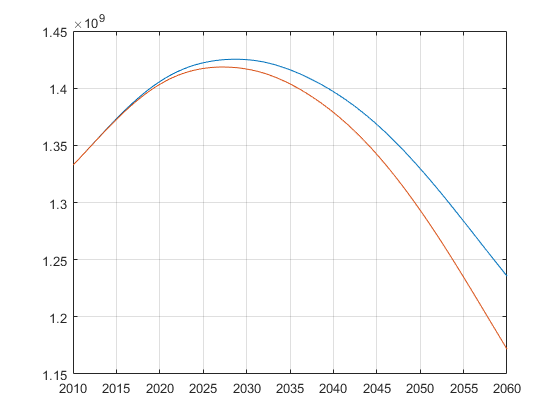
\includegraphics[width=10cm]{pics/amend_3.png}
		\caption{未来50年北京人口年龄分布预测比较}
		\*{(考虑城乡迁移与受教育水平提升)} \\
		\*{蓝线:若实施二胎政策} \\
		\*{红线:若未实施二胎政策}
		\label{amend_2_3}
	\end{figure}
	\begin{figure}
		\centering
		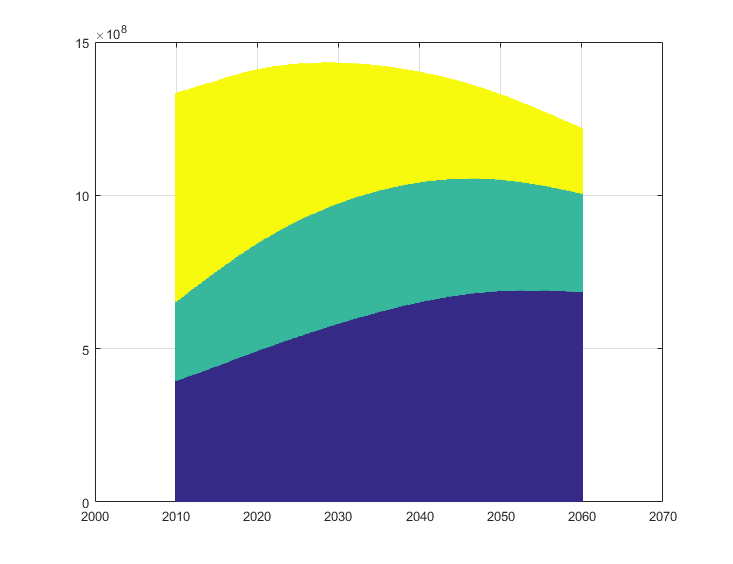
\includegraphics[width=10cm]{pics/amend_5.png}
		\caption{未来80年城镇乡的比例关系预测}
		\*{紫区:城市人口} \\
		\*{青区:镇人口} 	\\
		\*{黄区:农村人口}
		\label{amend_5}
	\end{figure}
\subsection{考虑计划生育政策的开放带来的影响}
\label{amend_section_3}
考虑到当二胎政策出台后,仅已生一胎的妇女生育意愿会增大,因此等式\ref{simple_birthrate}中$\beta_1(a, r_k, e_l)$将会比原来大,被修正为:
	\begin{equation}
		\label{amend_birthrate_policydown}
		\beta(a, r_k, e_l) = \eta_a \cdot \overline{\beta(a)} \cdot \lambda_i \cdot \lambda_b(k,l)
	\end{equation}
其中$\eta_a$是$a$岁已生育一胎的妇女在政策放开后的相对生育意愿。\\
\indent
据调查数据\footnote{国家计划生育委员会宣传司与北京零点指标信息咨询有限责任公司在2002年合作进行的生育意愿调查}显示:假若计划生育政策完全放开,那么各年龄阶层的妇女的平均期望生育孩子数将会上升。我们假定原来不愿意生育和愿意生育二胎的妇女意愿不发生变化(因为完全放开计划生育对她们没有实质性的影响),所以平均生育意愿数目的上升完全是来源于已生育一胎妇女的意愿改变。那么,设各年龄段平均期望生育孩子数目增加量为$\Delta n$,而期望生育两胎的妇女人数占比为$p_2(a)$;我们很容易地知道它们与$\eta_a$的关系是:
	\begin{equation}
		\label{amend_eta_a}
		\eta_a = 	\frac{\Delta n + p_2(a)}{p_2(a)}
	\end{equation}
根据数据,我们可以计算出$\eta_a$的分布情况:
	\begin{table}[H]
		\centering
		\caption{$\eta_a$的分布情况}
		\label{amend_eta_a_value}
		\begin{tabular}{c|ccccccc}
			\hline
			a的范围		&	[15,20)	&	[20,25)	&	[25,30)	&	[30,35)	&	[35,40)	&	[40,45)	&	[45,50)	\\
			\hline
			$\eta_a$	&	 2.241		&	1.931		&	1.677		&	1.621		&	1.621		&	1.733		&	1.705		\\
			\hline
		\end{tabular}
	\end{table}
对比计划生育政策开放前后人口结构情况,我们可以对政策的调整有一个大致的观念(图\ref{amend_4})。
	\begin{figure}[htbp]
		\centering
		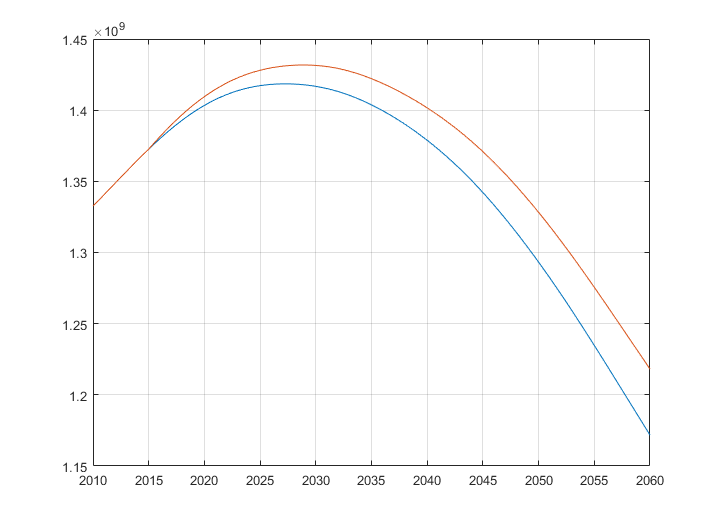
\includegraphics[width=10cm]{pics/amend_4.png}
		\caption{二胎政策开放前后中国人口趋势预测} 
		\*{蓝线:若未实施二胎政策} \\
		\*{红线:若实施二胎政策}
		\label{amend_4}	
	\end{figure}
\section{小结}
对比图\ref{amend_1}的红色曲线与图\ref{amend_4}中的红色曲线,我们可以明显地看到:如果认为生育第二胎的意愿与生育第一胎相同(去除政策阻力),那么中国人口将会缓步上升随后逐渐趋于稳定;但事实上,如果根据卫计委的生育意愿调查,那么中国人口同样会在2030年左右达到顶峰,随后人口数量发生萎缩。\\
\indent
我们选择使用节\ref{amend_section_3}的修正方案,是因为生育第二胎的意愿与生育第一胎的意愿是不能视为近似的。一个主要的原因是,生育第一胎的动力可以理解为是夫妻希望养育一个子女所驱动,但生育第二胎时非意愿生育($F_u$)将会起到主导作用。\\
\indent
“城镇育龄妇女与农村育龄妇女不想生二孩的主要原因都是养育成本高,分别占58.4\%和54.7\%。”\footnote{韩雷,田龙鹏:《“全面二孩”的生育意愿与生育行为——基于2014年湘潭市调研数据的分析》,《湘潭大学学报(哲学社会科学版)》第40卷第1期,第53页。}事实上,在温州,养一个孩子光是教育方面就要花40-80万元。\footnote{陈耀辉:《在温州养一个孩子要花多少钱》,《温州瞭望》2009年第5期,第66页}徐安琪也指出,“现代中国培养一个孩子要花49万元。” \footnote{徐安琪:《孩子的经济成本:转型期的结构变化和优化》,《青年研究》2004年第5期,第5页}这些数据都是在2010年之前得到的,而2010年至2015年的人均工资水平提高了70\%。所以如果我们按照这些费用均摊至20年,那么每年一个家庭要花费在孩子身上的费用要达到3.4万元(甚至可能远不止)。根据中国统计年鉴的数据,2015年平均工资收入为人均56360元,除去养老基金、社保、税金,一个家庭每年的可支配收入为65000元。这意味着大多数家庭是没有经济能力负担起抚养两个孩子的花销的;这也就是为什么模型计算所得开放二胎后人口数量并没有得到有效的补足,因为意愿会因为经济原因产生明显下滑。\\
\indent
尹豪曾指出,“就人口老龄化的进程而言,中国和韩国的情况比较接近。并且,在经济发展水平、社会状况以及文化背景等方面韩国同中国具有许多类似之处。”\footnote{尹豪:《韩国人口老龄化与老年人社会保障》,《人口学刊》2000年第5期,第31页}韩国人口政策的发展经历了控制人口数量的计划生育、调整出生婴儿性别比例以及鼓励生育三个阶段;然而,第三个阶段“新人口政策”的实施并没有带来补偿性生育高峰的出现,2003 年,韩国的总和生育率下降到了1.17,韩国不得不出台诸多鼓励生育的措施。\footnote{姚兴云、付少平:《韩国人口政策及其对中国农村人口政策的启示》,《西北人口》2009年第2期,第120页}\\
\indent
通过对于韩国的类比,我们可以发现,一段时间的控制人口所带来的后果并不是放开政策就可以解决的,甚至韩国十多年的鼓励生育政策也没有带来总和生育率的回升。乔晓春也总结发现了进入低生育水平国家的两条规律:无论政府是否干预,也不管当时的生育水平有多高,一旦经济发展到了一定水平,生育率都会自发下降;政府有能力让生育率下降,但很难做到让低生育率再度升高。\\
\indent
放开二胎仅仅是调控人口的第一步,接下来需要做的(例如鼓励生育政策,或者调控养育孩子的经济成本等)还有很多。
	
\part{报告研究}
\label{pipan}
\begin{quote}
\textit{“以上针对我国妇女生育意愿的多项调查结果均显示,目前妇女生育意愿仍处于较高水平,至少 60\%以上的妇女想要生育第二个孩子。但是,考虑到以往很多调查都是针对“单独”家庭的调查,而“单独”家庭多集中在城市,若全面放开二胎政策,很多农村家庭将进入政策覆盖范围,那么相应全国平均二胎生育意愿也会有所增加。因此,本文假定在立即全面放开二胎政策下,全国妇女二胎平均生育意愿为 70\%。”\\
“二胎生育意愿是随年龄上升而下降的,所以目标人群中的年龄结构会对出生数量产生影响”\\
“妇女时期总和生育率峰值可达4. 5左右”}\footnote{翟振武、张现苓、靳永爱:《立即全面放开二胎政策的人口学后果分析》,《人口研究》第38卷第2期,第10页}\\
\end{quote}
\indent
事实上,国家卫计委于2015年1月召开新闻发布会表示,2014年年中估计我国有符合申请单独二孩的家庭1100万对夫妻,提出申请生育二孩的夫妻应该有600万,但到 2014年年底为止,提出生育二孩申请的仅为100万,真正生育二孩的仅为50万左右,仅占当年生育数量(1687万)的3\%左右。2014年年底南京市卫计委受理“单独二孩”再生育家庭为9944例,实际办理9777例,但在2015年已经怀孕和已经生育的家庭仅为4223个(不足2014年出生人口的6\%),即怀孕生育妇女仅为预期人数的50\%左右。2015年7月国家卫计委开展的专项调查表明,仅有39.6\%的访者有再生二孩的打算。诸多数据表明(尤其是单独二孩开放后数据),全面二孩放开后的“生育意愿累积爆发”远不如预想得强烈,甚至可能连50\%都不及。\\
\indent
二胎生育意愿随年龄上升而下降也是错误的;相反地,根据之前所使用的计生委的调查数据,二胎生育意愿会随着年龄的上升而上升。但由于年龄的上升,怀孕几率下降、生育出婴儿抵抗力偏弱,导致二胎生育意愿偏高的高龄妇女并不能如愿产下二胎。这也是为什么之前预估人口爆炸式增长(迅速增长,至2018年后逐渐趋于平稳)不能实现的原因之一(这个预测与图\ref{amend_1}中的红色曲线更为接近,但这是理想状态,没有考虑到经济发展后生活水平提升导致的经济负担增加)。
\indent
根据节\ref{amend_section_3}中的二胎修正模型,我们可以得到总和生育率的图线如图\ref{amend_fertility_rate}。
	\begin{figure}[htbp]
		\centering
		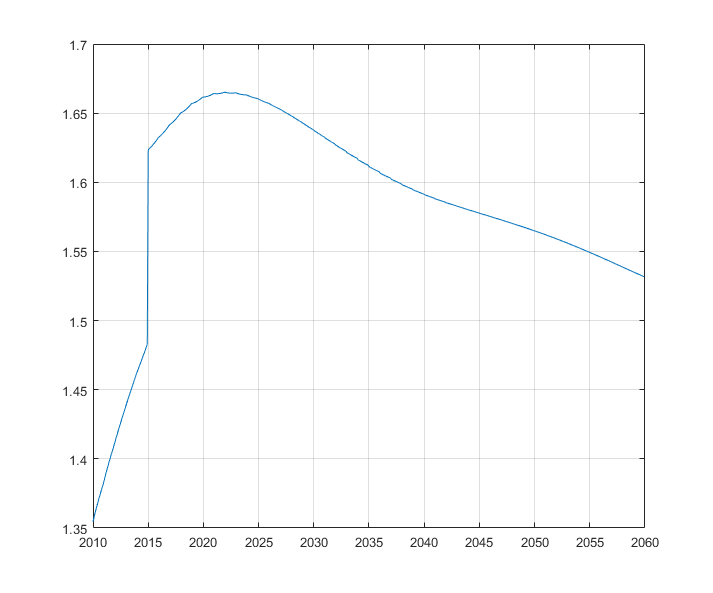
\includegraphics[width=10cm]{pics/amend_fertility_rate.png}
		\caption{总和生育率预测} 
		\label{amend_fertility_rate}	
	\end{figure}
\indent
可以看到,放开二胎政策后总和生育率的确会有瞬间地上升,但甚至没能超过1.7。即使再算上部分的生育意愿累计爆发,总和生育率也远达不到4.5。这说明这篇文献对于生育意愿的估计过高。\\
\indent
\begin{quote}
\textit{“文化程度低的被调查者希望生育较多的子女,随文化程度的不断提高,被调查者希望生育的子女数逐渐降低”\\
“文化程度高的人群对子女的未来期望值较高,更关心子女的质量,对子女教育的投入就更多,因此,对子女质量的要求就会取代数量的偏好。同时,由于教育的投入提高了养育子女的成本,在收入水平确定的条件下,生育的数量必然减少,因为在收入水平确定的情况下,多生育孩子,就必须减少子女的平均养育成本。”\footnote{周福林:《我国城乡居民分年龄、性别和受教育程度的生育意愿研究》,《西北人口》2005年第3期,第14页}}
\end{quote}
\indent
我们重新回到第\ref{simple_model}章所建立的简单模型中得到的修正参数矩阵。下面是利用2000年第五次人口普查的数据计算所得到的修正参数矩阵。
	\begin{table}[H]
		\centering
		\caption{由五普得到的生育修正参数$\lambda_b$}
		\label{simple_lambda_b_value_2000}
		\begin{tabular}{c|ccc}
			$\lambda_b(r_k,e_l)$	&	$e_0$	&	$e_1$	&	$e_2$	\\
			\hline
			$r_0$								&	0.750	&	0.746	&	0.605	\\
			$r_1$								&	1.072	&	0.885	&	0.817	\\
			$r_2$								&	1.390	&	1.018	&	0.794	\\
		\end{tabular}
	\end{table}
\indent
我们可以发现,相隔10年的数据所得到的修正参数矩阵有一定的差异,其中城市的修正参数基本持平,而乡镇高教育程度的妇女的生育意愿明显下降,乡村中等教育程度的妇女生育意愿上升。这并不意味着简单模型的偏差,而是因为2000年与2010年的教育程度、经济水平相差颇大。这个差异在近几年得到了有效的缓解(由于教育资源的日趋完善和房价等逐渐稳定),所以我们在之后的模型计算中使用了第六次人口普查所得到的修正参数矩阵。\\
\indent
而通过两次人口普查所得到的修正参数差异也是可以根据上面引用文献的话来解释的:城市的修正参数基本持平,是因为城市收入与教育支出稳步同比上升;乡镇高教育程度的妇女的生育意愿明显下降,是因为教育程度高的妇女对子女未来期望值高,但高程度教育的教育投入上涨远超过乡镇收入的上涨,所以生育意愿下跌;乡村中等教育程度的妇女生育意愿上升,是因为她们本身对于子女的未来期望值并不高,所以教育支出上涨幅度不大,但收入却有了不少的增长,于是生育意愿得到了提升。
	
\part{北京市的人口增长模型}
\section{数据的引用}
	\begin{table}[H]
		\centering
		\caption{近几年北京迁入人口数}
		\label{beijing_data}
		\begin{tabular}{c|cccccc}
			\hline
			年份				&	2010	&	2011	&	2012	& 2013	&	2014	&	2015	\\
			\hline
			迁入人口数	&	90.5		&	37.5		&	31.6		&	28.8		&	16.0		&	4.1		\\
			\hline
		\end{tabular}
	\end{table}
\section{模型的再次修正}
我们只要对等式\ref{amend_migrate}进行修正,加入外来人口的因素:
	\begin{equation}
		\label{beijing_amend_migrate}
		\sum_{e_l} N'''(a,r_0,e_l,t+1) = \sum_{e_l} N''(a,r_0,e_l,t+1) + M(a,t)
	\end{equation}
其中$M(a,t)$是$t$时间段内迁入北京市的$a$岁人口数目,$N'''(a,r_0,e_l,t+1)$是这一次修正后城市各受教育程度的人口数。\\\\
\indent
根据统计数据【来源请求】,在一个固定研究时间段内,$M(a,t)$随着$a$的分布如表\ref{beijing_migrate_rate}所示。如果假定在各年龄层迁入人口保持相同比例,那么,$M(a,t)$与总迁入人数$M(t)$的比例$\phi_a = \frac{M(a,t)}{M(t)}$满足如下关系:
	\begin{table}[H]
		\centering
		\caption{北京迁入人口随年龄的分布}
		\label{beijing_migrate_rate}
		\begin{tabular}{ccc}
			\hline
			年龄$a$分布	&	$\frac{\sum_a M(a,t)}{M(t)}$	&	$\phi_a$	\\
			\hline
			$[0,15)$			&	7.00\%	&	0.467\%	\\
			$[15,40)$		&	82.4\%	&	3.296\%	\\
			$[40,60)$		&	9.8\%		&	0.490\%	\\
			$[60,\infty)$	&	0.8\%		&	0.020\%	\\
			\hline
		\end{tabular}
	\end{table}
\indent
北京市总迁入人口$M(t)$,是基于历年的迁入人口(图\ref{beijing_1})拟合得出的:
	\begin{equation}
		\label{beijing_migrate_all}
		M(t) = M_0 + M_1 \cdot e^{-\kappa (t-t_0)}
	\end{equation}
其中参数拟合结果如表\ref{beijing_migrate_para}所示。
	\begin{figure}[htbp]
		\centering
		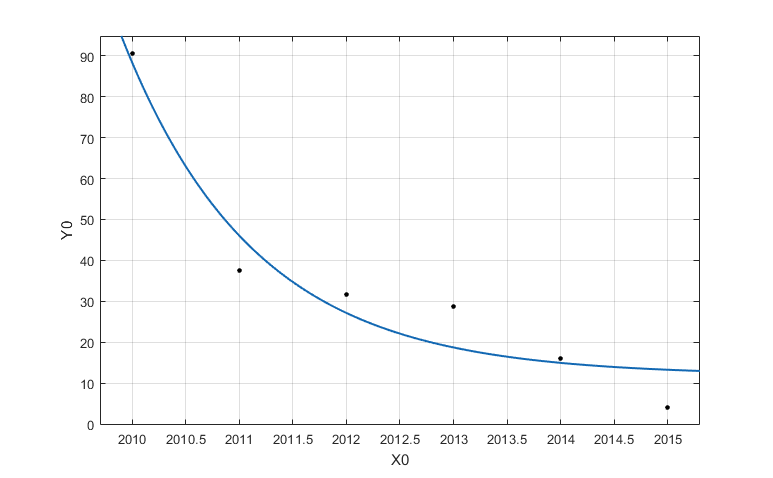
\includegraphics[width=10cm]{pics/beijing_1.png}
		\caption{北京近几年迁入人口数量拟合} 
		\label{beijing_1}	
	\end{figure}
	\begin{table}[H]
		\centering
		\caption{北京迁入人口参数拟合结果\ $t_0$=2010}
		\label{beijing_migrate_para}
		\begin{tabular}{c|ccc}
			参数	&	$M_0$	&	$M_1$	&	$\kappa$	\\
			\hline
			值		&	11.92 		&	76.43		&	0.8066		\\
		\end{tabular}
	\end{table}
\section{小结}
本章主要关注的是全国模型应用到北京这个地方模型上时会产生的“副作用”。很明显,对于北京而言,外来人口对于北京人口的构成起着不可忽视的作用;另一方面,北京的城市人口占到了总人口的近90\%【来源请求】,因此城镇化的过程并不需要过多的讨论。
	
\part{政策对社会造成的影响}
\section{未来人口数量与结构的预测}
\subsection{人口数量}
	\begin{figure}[htbp]
		\label{future_population_1}	
		\centering
		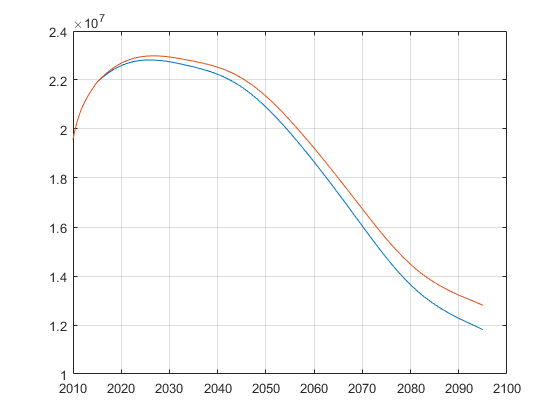
\includegraphics[width=10cm]{pics/future_population_1.png}
		\caption{2010-2095年北京人口数量预测}
		\*{蓝线:若未实施二胎政策} \\
		\*{红线:若实施二胎政策} 
	\end{figure}
对比图\ref{future_population_1}中的红线与蓝线可以发现二胎政策可以使得北京市总人口比计划生育政策下同期预测人口增长一些,至2090年可净增多10\%,但并没有改变北京市总人口在2025~2035年之间开始转增长为下降的趋势,说明二胎政策对于扭转中国人口回降与老龄化趋势的作用十分有限,因此在认为政府不再改变迁入政策(限制迁入)的情形下,我们认为北京市人口最高将在2025年左右达到2300万左右并开始下滑。
\subsection{人口随年龄的分布}
图\ref{future_age_1}、\ref{future_age_2}
	\begin{figure}[htbp]
		\centering
		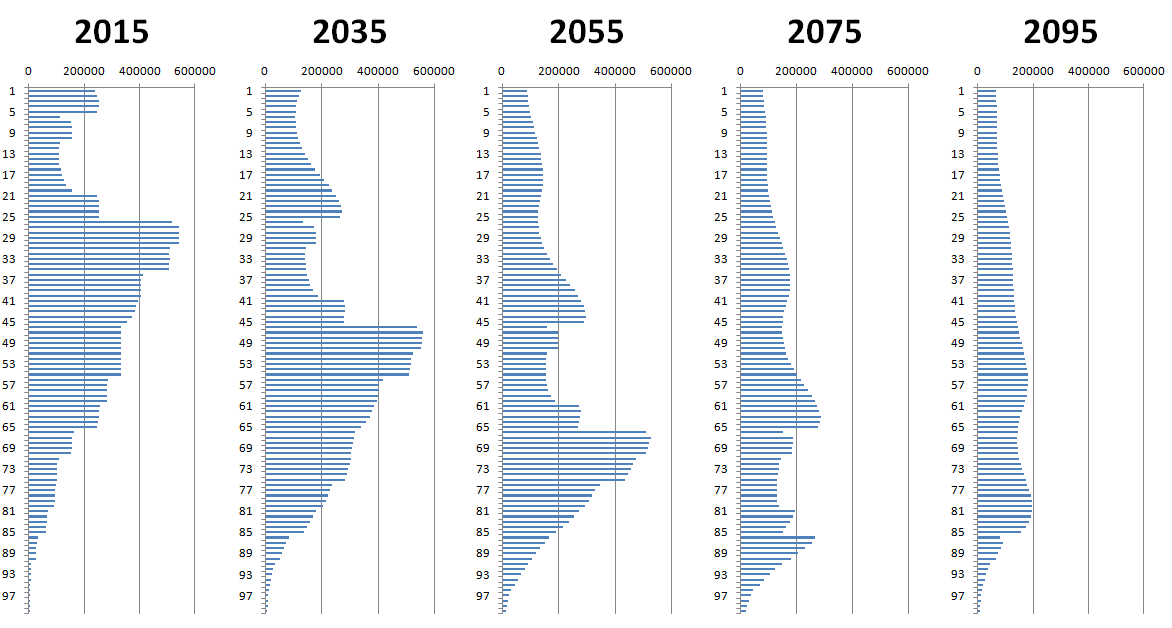
\includegraphics[width=10cm]{pics/future_age_1.png}
		\caption{2015、2035、2055、2075、2095年北京人口年龄结构预测 未开放二胎政策} 
		\label{future_age_1}	
	\end{figure}

	\begin{figure}
		\centering
		\subfigure[2035年]{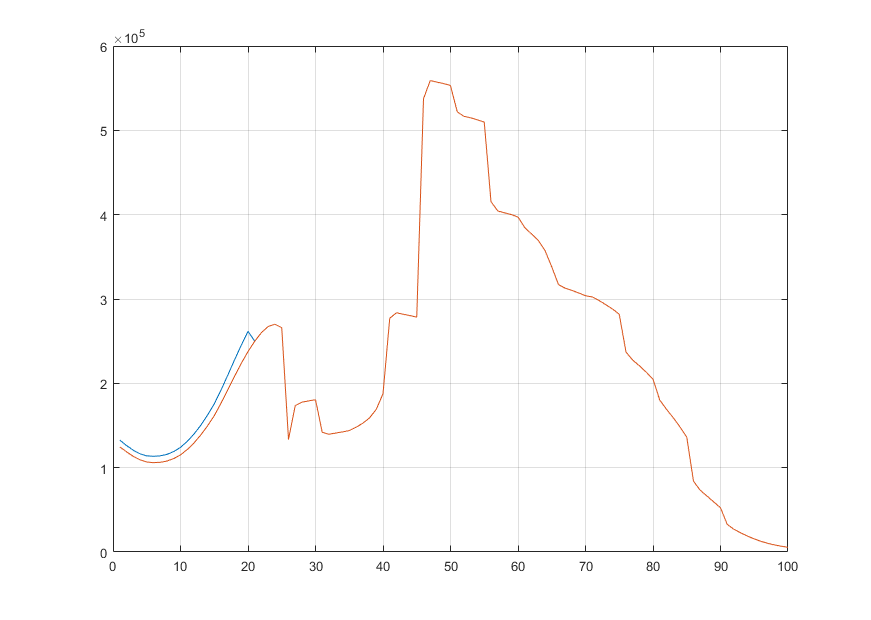
\includegraphics[width=5cm]{pics/future_age_35.png}}
		%\mbox{\hspace{0.5cm}}
		\subfigure[2055年]{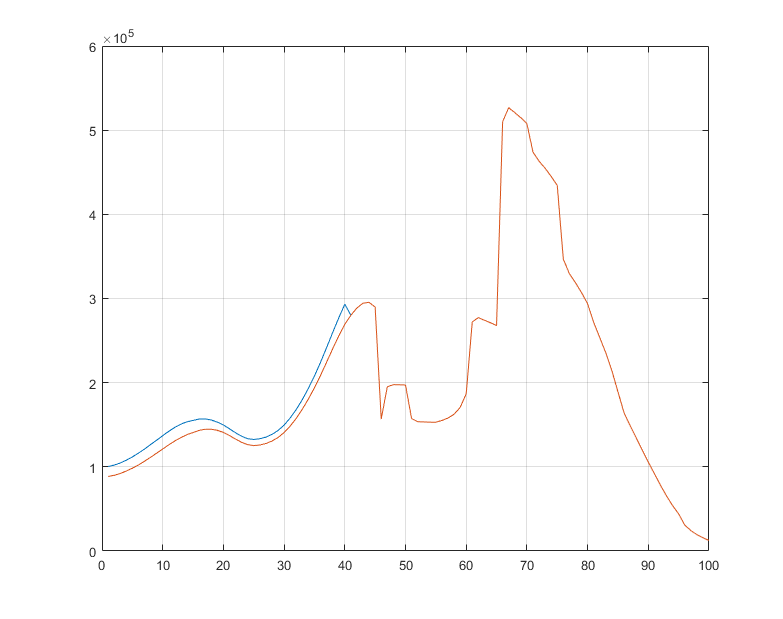
\includegraphics[width=5cm]{pics/future_age_55.png}}
		\\
		\subfigure[2075年]{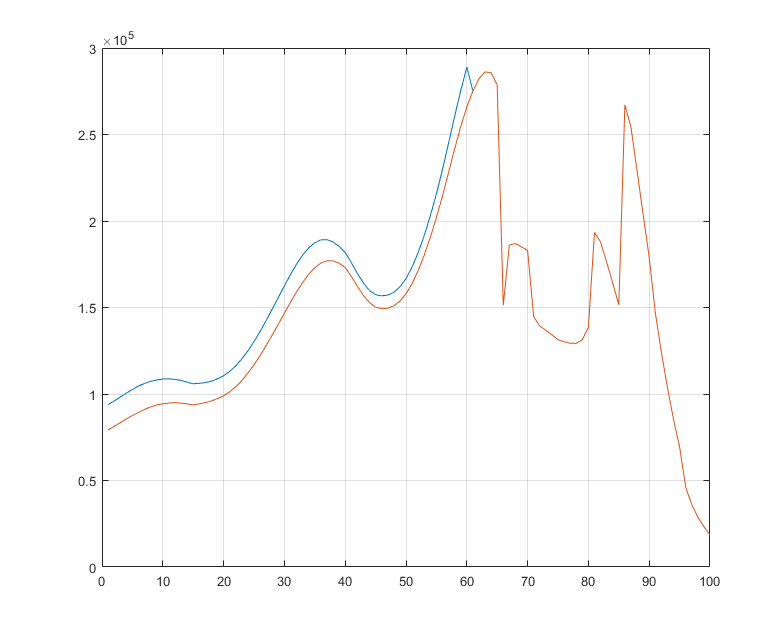
\includegraphics[width=5cm]{pics/future_age_75.png}}
		%\mbox{\hspace{0.5cm}}
		\subfigure[2095年]{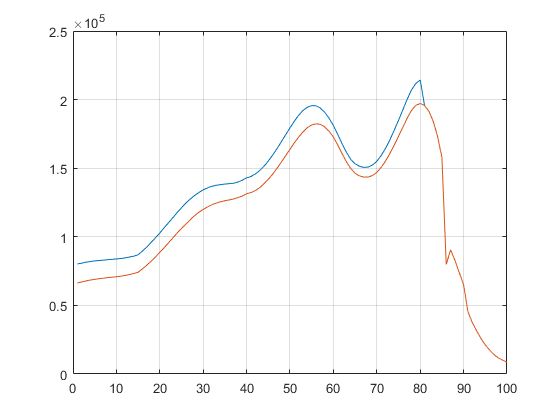
\includegraphics[width=5cm]{pics/future_age_95.png}}
		\caption{未来80年北京人口年龄分布预测比较}
		\*{蓝线:若实施二胎政策} \\
		\*{红线:若未实施二胎政策}
		\label{future_age_2}
	\end{figure}
由图\ref{future_population_1}我们得到由于二胎政策的实行使得生育率提高的程度十分有限,我们在分析北京市年龄结构随时间变化的时候可以忽略是否实行了二胎政策。通过图\ref{future_age_1}我们可以清晰地看到北京市人口在限制迁入政策下产生的人口老龄化过程,年龄峰值不断向高龄迁移。通过图中2015年部分我们可以看到北京市在2015年时人口绝大多数为年轻人(集中在25到37岁之间),可以认为产生这种情况的原因是2010年前相对宽松的北京市迁入政策,吸引了大量年轻人进京务工,进而形成了北京市在2015年独特的年龄层次结构(未成年人和老年人少,青壮年人多)。在2035年和2055年部分我们可以看到这一部分的人群在北京市依然占主导地位,但是其平均年龄相应延后,尤其值得注意的是2035年中17到21岁人群的小高峰和2055年对应的37到41岁人群的小高峰,这部分人群就是2015年中25到37岁之间人群的下一代。在2075年和2095年的部分中,2015中25到37岁之间的人群大部分已经死亡,2035年中17到21岁人群成为主导人群,但总体依然呈现老龄化和负增长,但老龄化程度较2035年和2055年有所下降。因此我们可以得到结论,在假定迁入政策(限制迁入)的情形下,北京人口逐渐步入老龄化,并在2055年左右达到老龄化的高峰;随着最初的主导人群的死亡,老龄化将有所缓解,但依然将保持老龄化的状态。
\subsection{受教育水平的分布变化}
图\ref{future_edu_pri_sen}
	\begin{figure}
		\centering
		\subfigure[高等教育]{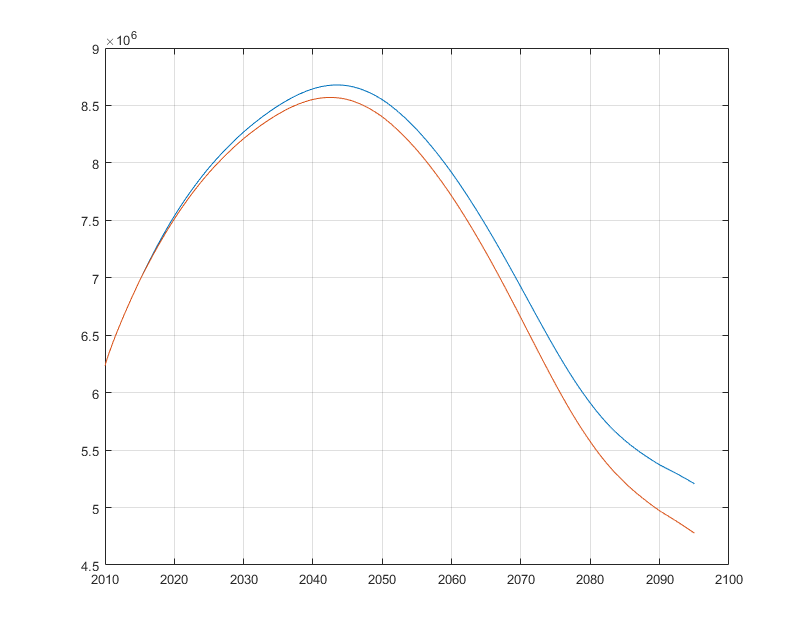
\includegraphics[width=5cm]{pics/future_edu_senior.png}}
		%\mbox{\hspace{0.5cm}}
		\subfigure[初等教育]{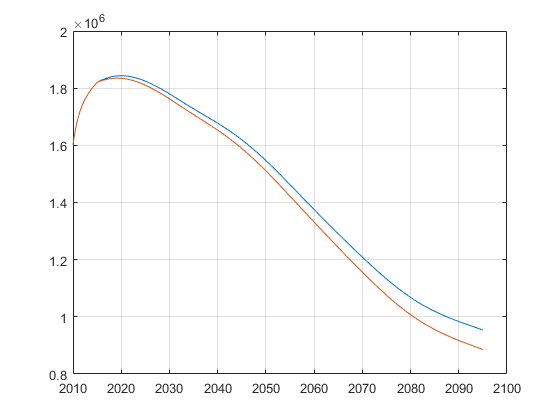
\includegraphics[width=5cm]{pics/future_edu_primary.png}}
		\caption{2010-2095年北京市受不同教育人口预测}
		\*{蓝线:若实施二胎政策} \\
		\*{红线:若未实施二胎政策}
		\label{future_edu_pri_sen}
	\end{figure}
由图\ref{future_edu_pri_sen}中的图(a)可知,由于教育水平迁移率的作用,北京市受高等教育的人口数将持续增长之二十一世纪中叶,但由于整体老龄化导致的人口负增长,受过高等教育的人口数量将快速下降(实际上比例并不会下降)。而由图(b)可知,初期(前五年)在大量外来人口涌入的作用下,北京市的初等教育人口呈短暂上升趋势,在2015年前后开始施行限制迁入政策后,在教育迁移的作用下初等教育人口数量开始下降,并在20世纪中叶由于整体人口负增长而开始加速下降。这两种趋势无论二胎政策的有无都是相同的。
\section{教育设施的压力}
考察7岁、12岁、16岁、19岁人口在是否开放二胎政策的人数差\ 图\ref{future_edu}
	\begin{figure}
		\centering
		\subfigure[7岁]{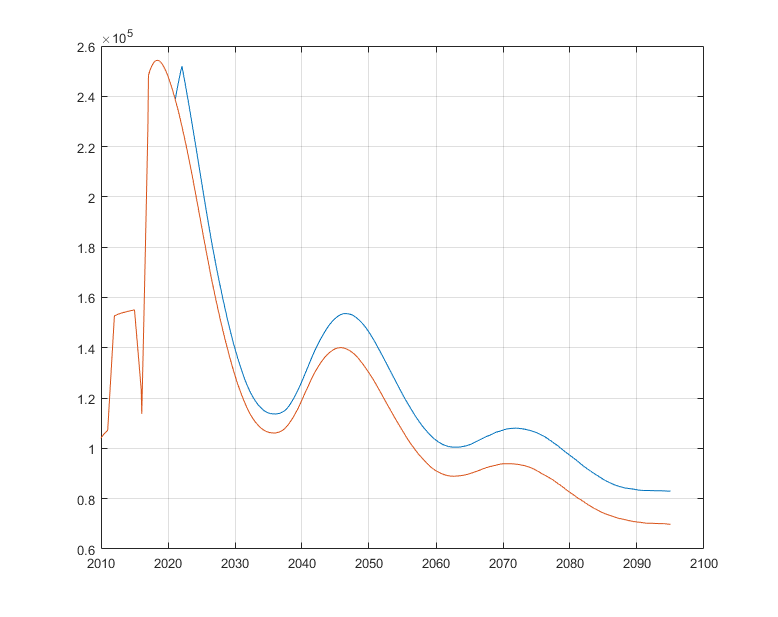
\includegraphics[width=5cm]{pics/future_edu_7.png}}
		%\mbox{\hspace{0.5cm}}
		\subfigure[13岁]{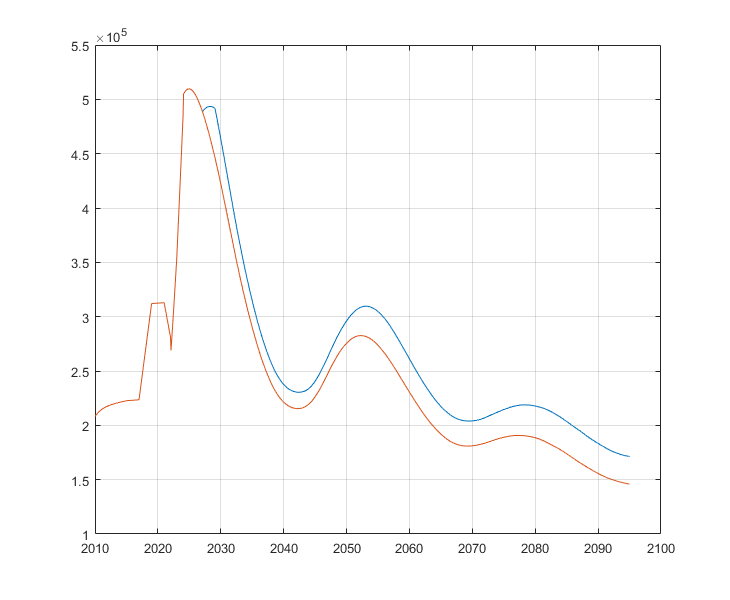
\includegraphics[width=5cm]{pics/future_edu_13.png}}
		\\
		\subfigure[16岁]{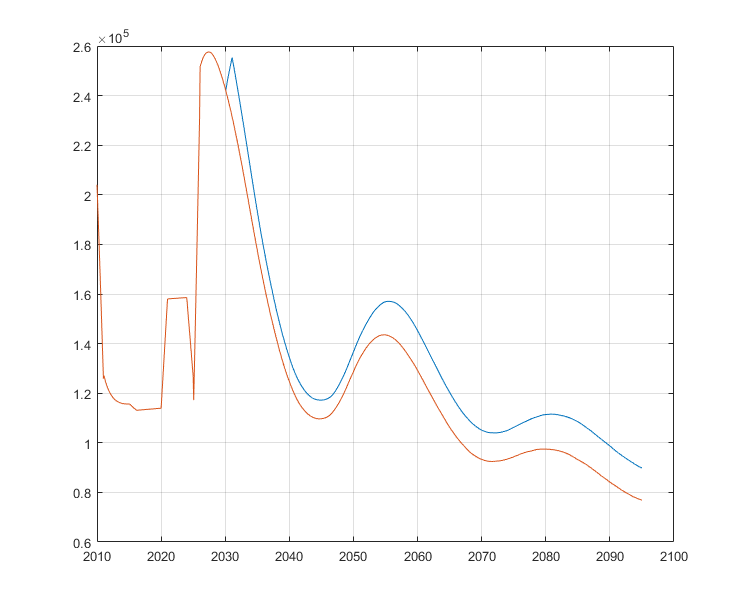
\includegraphics[width=5cm]{pics/future_edu_16.png}}
		%\mbox{\hspace{0.5cm}}
		\subfigure[19岁]{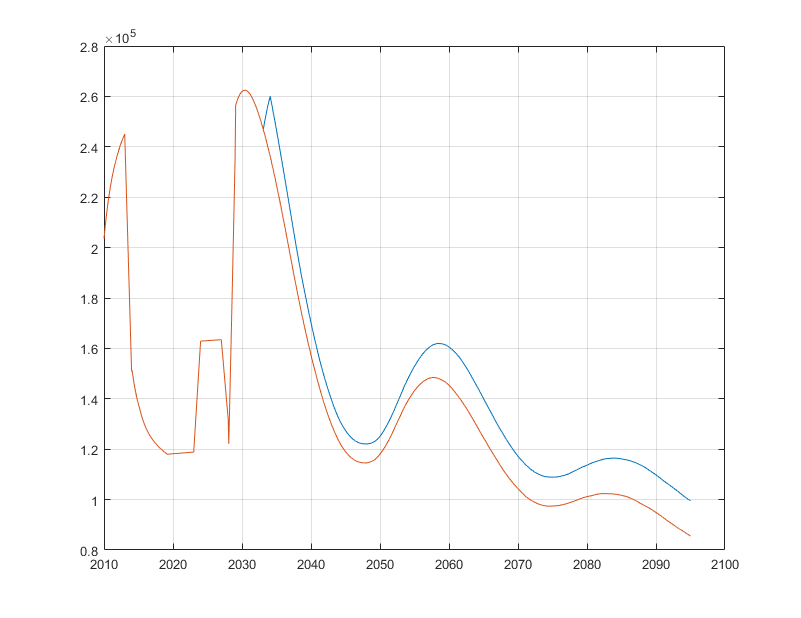
\includegraphics[width=5cm]{pics/future_edu_19.png}}
		\caption{未来80年北京特定年龄的青少年人数预测}
		\*{蓝线:若实施二胎政策} \\
		\*{红线:若未实施二胎政策}
		\label{future_edu}
	\end{figure}
通过图\ref{future_edu}可知对于计划生育政策下7岁、13岁、16岁和19岁的人群都会相应的迎来同一波入学高峰(小学在2017年前后,初中2023年前后,高中2026年前后,大学2029年前后),这一波高峰都是由于2015年前大量涌入的迁入人群的下一代产生的婴儿潮所引起的。对于放开二胎来说,相应的高峰推后五年会迎来第二个高峰,这个高峰是由于放开二胎所引起的婴儿数量上涨。同样由图像也可以得到,该人群的下一代产生的第二波婴儿潮同样会产生对教育系统的冲击(小学在2045年前后,初中在2051年前后,高中在2054年前后,大学在2057年前后),对于教育系统来说,届时应做好应对措施。
\section{劳动力供给与就业}
我们考虑从22岁值退休年龄前的青壮年人口,他们构成了北京市劳动力的主要部分。
而北京市的就业岗位数目,可以大致地从2010-2015年的数据中推算出来:就业人员占总人口的52\%-53\%;因此我们可以类似地预测接下来几年北京市就业岗位数目。
	\begin{figure}[htbp]
		\centering
		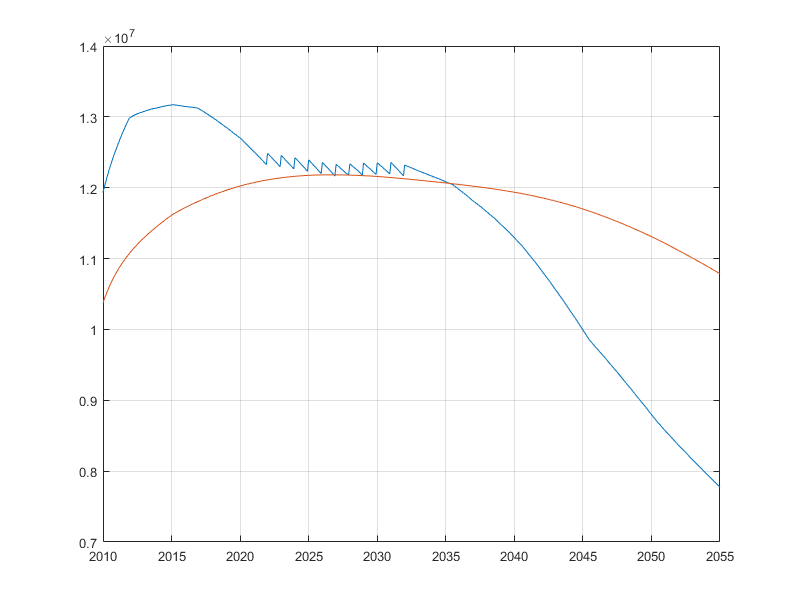
\includegraphics[width=10cm]{pics/future_work.png}
		\caption{未来北京劳动力供给与就业岗位预测} 
		\*{蓝线:劳动力人数(锯齿是由于推迟退休年龄造成的)} \\
		\*{红线:北京市工作岗位数}
		\label{future_work}	
	\end{figure}
图\ref{future_work}中我们可以得到北京市劳动力在2015年达到高峰之后便开始持续下降(主要由于迁入人口限制)。根据北京市的政策【来源请求】,将于2022年开始每年推迟6个月的退休时间,在图中可以看到如果不采取这样的措施,北京的劳动力将在2023年前后无法填补所有的工作岗位导致劳动力不足。通过推迟退休时间,北京市劳动力在2035年前都能满足工作岗位的需求,然而由于人口的老龄化,在2032年退休延迟政策停止之后,若不采取其它的措施,北京市的劳动力依然将于2035年开始不足。

\part{养老金模型}
在这一章中,不加特殊说明时,研究对象均为北京市与北京市人口。
\section{概述}
养老金,是“中国国营养老保险制”的民间俗称,本文亦沿用这一说法。中国国营养老保险制是中华人民共和国官方经营的养老保险,其经费归于社会保障基金下的社会保险基金项管辖投资运用。\footnote{维基百科编者. 中国国营养老保险制[G/OL]. 维基百科, 2015(20150403)[2016-05-02]. https://zh.wikipedia.org/w/index.php?title=\%E4\%B8\%AD\%E5\%9C\%8B\%E5\%9C\%8B\%E7\%87\%9F\%E9\%A4\%8A\%E8\%80\%81\%E4\%BF\%9D\%E9\%9A\%AA\%E5\%88\%B6\&oldid=34987840.}在参保过程中,无工作的个人缴纳金额以2014年整并的城乡居民养老保险为准,标准目前设为每年(人民币)100元、200元、300元、400元、500元、600元、700元、800元、900元、1000元、1500元、2000元12个档次,省区、市人民政府可以根据实际情况增设缴费档次,最高缴费档次标准原则上不超过当地灵活就业人员参加职工基本养老保险的年缴费额。参保人自主选择档次缴费,多缴多得。而领取给付时分为基础养老金与个人账户养老金两部分。\\
\indent
为了简化模型,我们暂且仅考虑某一个基准年度养老金的发放水平,与政府给出的每年养老金补贴比例;并且使用平均收入代表总人口的收入水平。
\section{符号表}
	\begin{table}[H]
		\centering
		\caption{养老金模型符号表}
		\label{pension_symbol}
		\begin{tabular}{ccc}
			\hline
			符号				&	含义	\\
			\hline
			$F(t)$				&	$t$时间国家养老基金的已有积累			\\
			$F_i(t)$			&	$t$时间段养老基金的收入						\\
			$F_o(t)$			&	$t$时间段养老基金的支出						\\
			$N_i(t)$			&	$t$时间段上缴养老保险金的人数			\\
			$N_o(t)$			&	$t$时间段领取养老金的人数					\\
			$P(t)$				&	每年养老金发放给个人的金额				\\
			$C(t)$				&	每年单个参保人员需要缴纳的保险金	\\
			\hline
		\end{tabular}
	\end{table}
\section{数据的引用}
		\begin{table}[H]
		\centering
		\caption{养老金数据}
		\label{pension_data}
		\begin{tabular}{ccc}
			\hline
			参数				&	值			&	含义 \\
			\hline
			$t_0$				&	2015		& 数据统计年	\\
			$F(t_0)$			&	1150		&	北京养老基金初始积累/亿元	\\
			$P_0$				&	3050		&	$t_0$年养老金平均发放金额/元	\\
			$S_0$				&	7109		&	$t_0$年人均收入/元	\\
			$S_u$				&	120			&	每年政府补贴养老基金的总额/亿元	\\
			$\gamma_i$	&	1.1			&	物价水平上涨指数	\\
			$\gamma_p$	&	1.065		&	养老金上调幅度	\\
			$\gamma_s$	&	1				&	补贴随通货膨胀而产生的折合率(即补贴不随着时间变化)	\\
			$\theta_p$	&	8\%			&	养老金征收比例	\\
			\hline
		\end{tabular}
	\end{table}
\section{模型的建立}
我们从养老金的支出与收入两方面来看待养老金的流动。对于$t$时间国家养老基金的已有积累,采用记号$F(t)$。
\subsection{支出}
养老基金的支出,即为给符合条件的老龄人口的发放。为了简化问题,我们并不考虑养老金与退休人员的年龄之间的关系;亦即,退休人员在同一年中获得相同的养老金。考虑$t$时间段养老基金的减少量$F_o$:
	\begin{equation}
		\label{pension_out}
		F_o(t) = N_o(t) \cdot P(t)
	\end{equation}
其中$N_o(t)=\sum_{A_R(t) \leq a} N(a,t)$是所有符合退休条件的人数,$P(t)$是养老金发放的金额。\\\\
\indent
而养老金的发放金额,根据【来源请求】,是由一个基准量加上修正而得到的;我们可以依此列出方程:
	\begin{equation}
		\label{pension_per_out}
		P(t) =  P_0 \cdot \gamma_p^{t-t_0}
	\end{equation}
其中$P_0$是$t_0$年养老金发放的平均水平,$\gamma_p$是养老金上调幅度。
\subsection{收入}
养老基金的收入,主要依赖于企事业员工定期缴纳的养老保险金。类似的,我们并不考虑缴纳人员的收入差异,而使用他们的平均工资代替。那么,
	\begin{equation}
		\label{pension_in}
		F_i(t) = N_i(t) \cdot C(t) + S_u \cdot \gamma_s^{t-t_0}
	\end{equation}
其中$N_i(t)=\sum_{A_W(t) \leq a < A_R(t)} N(a,t)$是所有符合缴纳保险金的人数,$C(t)$是单个参保人员需要缴纳的保险金,$S_u$是每年政府补贴养老基金的总额,$\gamma_s$是补贴随通货膨胀而产生的折合率。\\\\
\indent
而单个参保人员需要缴纳的保险金,根据【来源请求】,是根据其收入与生活物价水平综合计算而得的;于是
	\begin{equation}
		\label{pension_per_in}
		C(t) = S_0 \cdot \gamma_i^{t-t_0} \cdot \theta_p
	\end{equation}
其中$S_0$是$t_0$年人均收入,$\gamma_i$是物价水平上涨指数,$\theta_p$是养老金征收比例。
\subsection*{小结}
因此,综合以上两方面,我们写出养老基金积累的递推关系:
	\begin{eqnarray}
		\label{pension_io}
		F(t+1) &=& F(t) - F_o(t) + F_i(t) \\
					&=& \sum_{A_R(t) \leq a} N(a,t) \cdot P_0 \cdot \gamma_p^{t-t_0} \nonumber \\
					&+& \sum_{A_W(t) \leq a < A_R(t)} N(a,t) S_0 \cdot \gamma_i^{t-t_0} \cdot \theta_p
	\end{eqnarray}
\section{数据的预测}
我们先观察在现行情况下,养老基金的收入(不考虑政府补贴)与支出情况(图\ref{pension_io})。
	\begin{figure}[htbp]
		\centering
		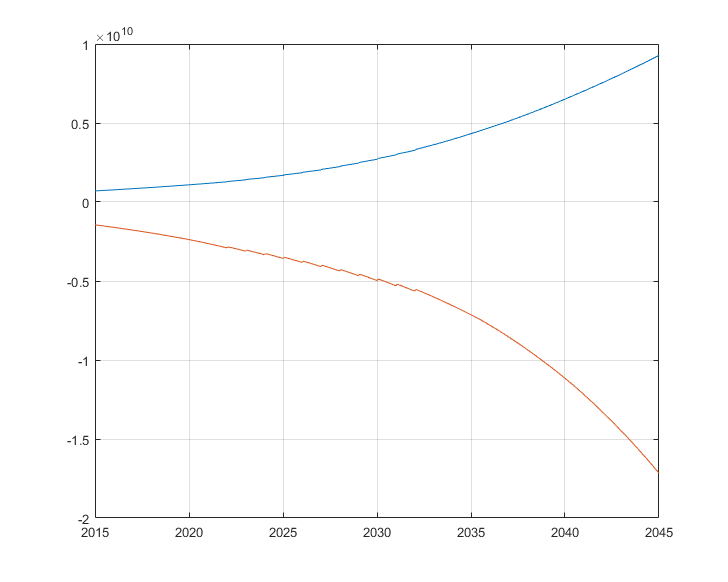
\includegraphics[width=10cm]{pics/pension_io.png}
		\caption{现行计划生育政策下养老基金收入与开支对比} 
		\*{蓝线:收入(不考虑政府补贴)} \\
		\*{红线:支出发放}
		\label{pension_io}	
	\end{figure}
我们再观察如果有政府补贴,对比二胎政策出台与否,养老基金总积累的变动情况(图\ref{pension_accu})。
	\begin{figure}[htbp]
		\centering
		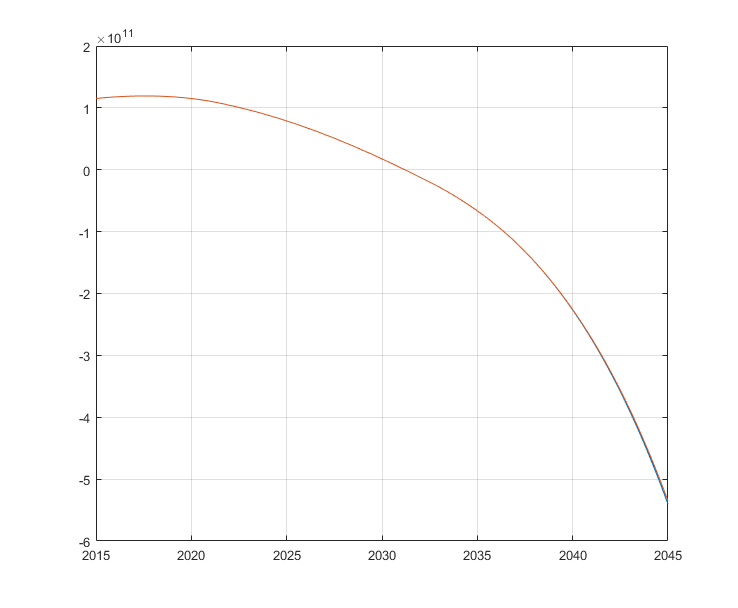
\includegraphics[width=10cm]{pics/pension_accu.png}
		\caption{比较开放二胎政策与否养老基金总积累的变动情况} 
		\*{蓝线:若未实施二胎政策} \\
		\*{红线:若实施二胎政策}
		\label{pension_accu}	
	\end{figure}
鉴于二胎政策是否出台对于养老金问题影响实在太小,所以下面并不区分这两种情况。
考虑增加政府补贴的折合率,即不同的$\gamma_s$	是否有可能避免养老基金的负值(图\ref{pension_gamma_s})。
	\begin{figure}[htbp]
		\centering
		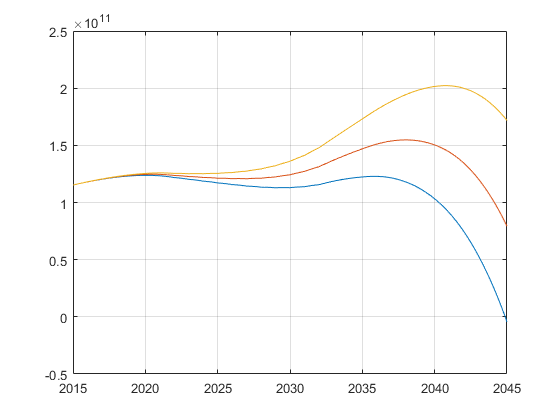
\includegraphics[width=10cm]{pics/pension_gamma_s.png}
		\caption{调整$\gamma_s$,考察养老基金的积累状况} 
		\*{黄线:$\gamma_s$ = 6.5\%} \\
		\*{红线:$\gamma_s$ = 6.0\%} \\
		\*{蓝线:$\gamma_s$ = 5.5\%} 
		\label{pension_gamma_s}	
	\end{figure}
\section{小结}
从图\ref{pension_accu}中,我们几乎不能够察觉二胎政策的实施带给养老金模型的影响;这种情况正是模型建立之初就可以预知的。因为一代人对养老金的影响仅仅在他们开始工作,并缴纳保险金的时候才体现出来;而从二胎政策的推行到影响的显现至少需要二十年的时间。除此以外,我们还必须注意到,二胎政策并不能大福影响人口的增长;所以综合以上分析,我们对于二胎政策能够缓解养老基金的短缺这一说法持怀疑态度。\\
\indent
养老基金短缺这一问题也许是能够通过提升政府补贴额度而得到解决的:从图\ref{pension_gamma_s}中我们可以知道,如果政府补贴折合率达到$\gamma_s$ = 6.0\%,就和有可能避免养老基金的耗尽。这是一条比调整人口或是减少发放更为行之有效的途径。
\part{总结}
开展计划生育的30年来,经济水平飞速发展,但与此同时也迎来了总和生育率严重下滑、人口老龄化严重的问题。虽然全面放开二孩政策可以缓解人口年龄比例失调,但类比于韩国对于调控人口的鼓励政策我们可以发现,仅仅是放开之前的政策约束并不能有效地弥补之前由于计划生育所少出生的那部分人口缺口。我们在马瀛通的年龄-孩次模型基础上考虑不同地区与不同教育程度对于妇女生产意愿的影响,得到了最终的修正二胎模型。可以发现,如果人们对于生育二胎的意愿和对于生育一胎的意愿类似的话,中国的人口总量将会短期内快速增长,随后减缓增长速率趋于稳定;但由于随着时间的推移,国人教育水平的提升以及抚养孩子经济压力的增大,妇女们生育孩子的主观意愿有所下降,客观条件又限制了她们生育二胎的可能性,所以放开二胎政策在近50年来看并没有明显的改观,人口总量在2030年左右达到峰值后又会骤跌。放开二孩政策只是政府调控人口的第一步,出台政策鼓励生育以及发展经济,让国民有更富裕的能力去抚养多个孩子才是当务之急。\\
\indent
而二胎开放对于北京市的影响更是显得微不足道。事实上,由于北京市大多为城市人口,而城市人口的生育意愿修正参数均小于1,外加上由于北京市政府为了限制2030年北京市人口不超过2300万人而限制了外来人口来京务工,这便导致了北京市劳动力得不到足够的补给,而人口老龄化又迅速来到。本身开放二胎对于城市的影响幅度是最小的,而且开放二胎对于北京的潜在支撑比(劳动力人数除以老年人数)的影响要至少经过20年才得以体现,但20年后老龄化已经极具严重,养老基金业逐渐体现赤字,所以希望通过二胎开放政策来调节人口老龄化和劳动力供给不足是不现实的。一个治标不治本的办法是增大政府养老金的补贴数额,但这同样不能解决劳动力供给不足的问题。在2035年退休年龄确定后,北京的人数已经大幅下降,不再出于半饱和状态,所以一个行之有效的方法是尽快鼓励生育或者是在之后北京人口数量下降时鼓励外来人口迁入。

\part*{参考文献}


\end{document}
